
\section{Analyse des propriétés des signaux physiologiques}

\begin{obj}
Analyser les propriétés des signaux physiologiques et en déduire des éléments du cahier des charges
de la loi de commande pour assurer le déplacement du robot avec le niveau de précision requis.
\end{obj}


\subsection{Analyse des propriétés des signaux des mouvements physiologiques}

\begin{obj}
Proposer un algorithme permettant de mettre en évidence les propriétés des mouvements respiratoires.
\end{obj}
\question{} ~\\ %Q1 --

%\textbf{Proposition 1}
%
%En première approximation, on peut dire que ce signal est périodique, de période \SI{4,8}{s}. La valeur maximale est de \SI{5}{mm} et la valeur minimale est de \SI{-2,5}{mm} soit une amplitude de .
%Si on avait à la modéliser par un signal sinusoïdal on aurait $e(t)=3,75 \sin\left(\dfrac{2\pi}{4,8} t\right) + 1,25$.
%
%\textbf{Proposition 2}
Le signal semble presque periodique même si les amplitudes des déplacements ne sont pas exactement les mêmes.
L'amplitude maximale obtenue est d'environ $\dfrac{5+2,3}{2}=\SI{3,65}{mm}$ et l'amplitude minimale obtenue est d'environ : $\dfrac{4+2}{2}=\SI{3}{mm}$. 
La période des oscillation est d'environ $
T\approx\dfrac{41-4}{9}\approx \SI{4,1}{s}$. 
Soit une pulsation de $\omega\approx \SI{1,53}{rad.s^{-1}}$.


\question{} %Q2 --
D'après la définition, 
$\hat{S}\left( f_n\right)= \dfrac{1}{N_f} \sum \limits_{k=0}^{N_f-1} s\left[kT_e\right] \text{e}^{-i 2 \pi f_nT_e k}$

$= \dfrac{1}{N_f} \left(
 s\left[0 T_e\right] \text{e}^{-i 2 \pi f_nT_e 0} + 
 s\left[T_e\right] \text{e}^{-i 2 \pi f_nT_e } + ... 
 s\left[\left( N_f-1\right)T_e\right] \text{e}^{-i 2 \pi f_nT_e \left( N_f-1\right)}\right)$

$= \dfrac{1}{N_f} \left(
 s\left[0\right] + 
 s\left[T_e\right] \text{e}^{-i 2 \pi f_nT_e } + ... 
 s\left[\left( N_f-1\right)T_e\right] \text{e}^{-i 2 \pi f_nT_e \left( N_f-1\right)}\right)$.
 
 On a donc $l_k\left(f_n\right)=\dfrac{1}{N_f}\text{e}^{-i 2 \pi f_nT_e k}$.
 

\question{} %Q3 --

On a $L_n = \begin{pmatrix}  l_0 f_n  & l_1 f_n & l_2 f_n & \ldots & l_{N-1} f_n\end{pmatrix}$.
Par ailleurs, 
$S_p = 
\begin{pmatrix} \hat{S}\left( 0\right) \\ \hat{S}\left( f_1\right) \\ \hat{S}\left( f_2\right)  \\ \vdots \\ \hat{S}\left( f_{N-1}\right) \end{pmatrix} 
=
\begin{pmatrix} 
L_0 V_s \\
L_1 V_s \\
L_2 V_s \\
\vdots \\
 L_{N-1} V_s\end{pmatrix}$.

On a donc $ L_{k} V_s =\begin{pmatrix}  l_0 f_k  & l_1 f_k & l_2 f_k & \ldots & l_{N-1} f_k\end{pmatrix} \begin{pmatrix}
s[0]  \\ s[T_e] \\ s[2T_e] \\ \vdots \\ s\left[\left(N-1\right)T_e\right] \\   \end{pmatrix} = \sum  \limits_{i=0}^{N-1} l_i f_k s\left[i T_e\right]$.


Ainsi la matrice $M$ est composé de toutes les lignes $L_n$ pour $n\in  \llbracket 0,N_f-1\rrbracket$.
La matrice $M$ aura donc pour forme : 

$
M=\dfrac{1}{N_f}
\left(
\begin{array}{cccc}
1 & 1 & \ldots & 1 \\ 
1 & e^{-i2\pi f_1T_e} & \ldots & e^{-i2\pi f_{1}T_e(N-1)} \\ 
\vdots & e^{-i2\pi f_nT_e} & \ldots & e^{-i2\pi f_{n}T_e(N-1)} \\ 
1 & e^{-i2\pi f_{N_f-1}T_e} & \ldots & e^{-i2\pi f_{N_f-1}T_e(N-1)} \\ 
\end{array} 
\right)
$.



\question{} %Q4 --
De la question précédente, on peut exprimer le terme $a_{n,m}$  : 

$a_{n,m}=\dfrac{1}{N_f}e^{-i2\pi f_{n}T_em}$.


\question{} %Q5 --

En posant 
$
X=-i2\pi
\left(
\begin{array}{c}
0\\
f_1\\
f_2\\
\vdots\\
f_{N_f-1}
\end{array}
\right)
\cdot
\left(
\begin{array}{ccccc}
0& T_e & 2T_e &\ldots & (N-1)T_e
\end{array}
\right)
=-i2\pi E_f\cdot t_k
$, on obtient bien, $
M=\dfrac{1}{N_f}\exp(X)$.

\question{} %Q6 --
%\begin{py}
\begin{lstlisting}
import numpy as np
def calculSpectre(Signal,Nf,fmax,Te):
    Vs=np.transpose([np.array(Signal)])
    Ef=np.transpose([np.linspace(0,fmax,Nf)])
    tk=np.array([range(len(Signal))])*Te
    X=np.dot(Ef,tk)*(-1j*2*np.pi)
    M=1/Nf*np.exp(X)
    Sp=np.dot(M,Vs)
    An=abs(Sp)
    return An
\end{lstlisting}
%\end{py}

\subsection{Cahiers des charges partiel de la chaîne d'asservissement en position du robot esclave}

\begin{obj}
Déterminer une valeur numérique pour la bande passante de l’asservissement en position du robot
esclave et vérifier le cahier des charges associé.
\end{obj}

\question{}	 %% Q7 --

D'une part, $H(p)=\dfrac{\varepsilon (p)}{Z^*(p)}$ et d'autre part, $F(p)=\dfrac{Z (p)}{Z^*(p)}$. Enfin, $\varepsilon(p)=Z^*(p)-Z(p)$. On a donc $\varepsilon(p)=\dfrac{\varepsilon(p)}{H(p)} - F(p)Z^*(p)=\dfrac{\varepsilon(p)}{H(p)} - F(p)\dfrac{\varepsilon(p)}{H(p)}$. On a donc  $\varepsilon(p)=\dfrac{\varepsilon(p)}{H(p)} - F(p)\dfrac{\varepsilon(p)}{H(p)} \Leftrightarrow $ $H(p)=1 - F(p)= p\dfrac{p+2\xi\omega_0  }{p^2+2\xi\omega_0 p + \omega_0^2}$.


En mettant cette fonction de transfert sous forme canonique, on  obtient : 
$
H(p)=\dfrac{2\xi\cdot p}{\omega_0}\dfrac{1+\dfrac{p}{2\xi\omega_0}}{1+\dfrac{2\xi}{\omega_0}p+\dfrac{p^2}{\omega_0^2}}
$.

\begin{itemize}
\item Le module de cette fonction de transfert en remplaçant $p$ par $i\omega$ représente le rapport des amplitudes en régime permanent vis-à-vis d'une entrée $z^*(t)$ sinusoïdale : 
$
\dfrac{\varepsilon_2}{A_2}=\Vert H(i\omega_2)\Vert
$.
\item L'argument de cette fonction de transfert en remplaçant $p$ par $i\omega$ représente le déphasage en régime permanent vis-à-vis d'une entrée $z^*(t)$ sinusoïdale : 
$
\Theta_2-\Phi_2=\arg\left(H(i\omega_2)\right)
$.
\end{itemize}

Ainsi on a : 
$
\left\{
\begin{array}{c}
\varepsilon_2=A_2\cdot \Vert H(i\omega_2)\Vert\\
\\
\Theta_2=\arg\left(H(i\omega_2)\right)+\Phi_2
\end{array}
\right.
$.


%Supposons que  $z_2(t)=A_2\sin \left(\omega_2 t + \Phi_2 \right)$. De plus, $\varepsilon_2(t)=\varepsilon_2 \sin \left( \omega_2 t + \Theta_2 \right)$. On a donc, $\varepsilon_2 = || H\left( i\omega_2\right)|| A_2$, $\Phi_2 - \Theta_2 = \arg \left(H\left(i\omega_2\right)\right)$.







\begin{rem}
Il est peut être souhaitable de préciser avant la question aux candidats qu'on a $z_n(t)=A_n\sin \left(2\pi f_n t + \Phi_n \right)=A_n\sin \left(\omega_n t + \Phi_n \right)$. 
\end{rem}

\question{}	 %%Q8 --
%Lorsque $\omega << \omega_0$, $\left|\left|  \dfrac{1}{p^2+2\xi\omega_0 p + \omega_0^2} \right|\right|$ tend vers 0. Calculons $\left|\left|  \left( j \omega \right) ^2+2\xi\omega_0  \omega j  \right|\right| =\sqrt{4\xi^2\omega_0^2 \omega^2 + \omega^2} =\omega \sqrt{4\xi^2\omega_0^2  + 1}$. 
%
%On a donc $|| H\left( i\omega\right)|| \simeq K\omega $ avec $K=\sqrt{4\xi^2\omega_0^2  + 1}$ lorsque $\omega << \omega_0$.
%
%\textcolor{red}{A VERIFIER Au final, $\varepsilon_2 \simeq \omega_2 \sqrt{4\xi^2\omega_0^2  + 1} A_2\sin \left(\omega_2 t + \Phi_2 \right) $.}

En considérant de faibles pulsations telles que $\omega\ll \omega_0$, on peut effectuer l'approximation : 
$\Vert H(i\cdot \omega)\Vert\approx\dfrac{2\xi\omega}{\omega_0}$.

On obtient donc bien : $\Vert H(i\omega)\Vert\approx K\cdot \omega $  avec $K=\dfrac{2\xi}{\omega_0}$.

On a alors $\varepsilon_2=A_2\cdot \Vert H(i\omega_2)\Vert $ $\simeq A_2 \dfrac{2\xi}{\omega_0}\omega_2$

\question{}	~\\
D'après l'exigence 1.3.3, $\dfrac{\varepsilon_2}{A_2}<10^{-2}$, on obtient alors la relation suivante : $
\dfrac{\varepsilon_2}{A_2}\approx \dfrac{2\xi\omega_2}{\omega_0}<10^{-2}$.  

Ce qui donne $\omega_0>200\xi\omega_2\approx \SI{603}{rad.s^{-1}}$

L'exigence 1.2 du cahier des charges concernant l'asservissement en position, et donc la fonction de transfert $F(p)$, impose une bande passante (que l'on suppose à $\SI{0}{dB}$), inférieure à $\SI{30}{rad.s^{-1}}$. $F(p)$ est une fonction de transfert du second ordre de gain 1 et la bande passante à $\SI{0}{dB}$ est de l'ordre de $\omega_0\approx \SI{600}{rad.s^{-1}}$. \textbf{Le cahier des charges est donc bien respecté.}


% Piste 2 Calculons $\omega_{BP}$ tel que $||F\left(j\omega_{BP}\right)|| = 0$ : 
%$\left|\left|F\left(j\omega\right)\right|\right|$ 
%$=\left|\left| \dfrac{\omega_0^2}{\omega_0^2-\omega^2+2\xi\omega_0\omega j} \right|\right|$

% $=\left|\left| 
% \dfrac{
% \omega_0^2 \left(\omega_0^2-\omega^2-2\xi\omega_0\omega j \right)
% }{
% \left( \omega_0^2-\omega^2+2\xi\omega_0\omega j\right) \left(\omega_0^2-\omega^2-2\xi\omega_0\omega j\right)}  % \right|\right|$
% $=\left|\left| 
% \dfrac{
% \omega_0^2 \left(\omega_0^2-\omega^2-2\xi\omega_0\omega j \right)
% }{
%  \left(\omega_0^2-\omega^2\right)^2 +4\xi^2\omega_0^2\omega^2 
% }  \right|\right|$

% Piste 1Supposons que $\dfrac{\varepsilon_2}{A_2} < 10^{-2}$ (exigence 1.3.2), on a alors $  \sqrt{4\xi^2\omega_0^2  + 1} \sin \left(\omega_2 t + \Phi_2 \right) < 10^{-2} $ 
% $\Rightarrow  \sqrt{4\omega_0^2  + 1} \sin \left(\omega_2 t + \Phi_2 \right) < 10^{-2} $.

%\textbf{Remarque :} je ne comprends pas bien la formulation de la question : << En considérant $\varepsilon_2$, déterminer (...) >>.


\section{Analyse géométrique et élaboration du modèle dynamique du robot esclave}

\begin{obj}
Vérifier la capabilité du robot esclave à respecter le cahier des charges et déterminer le modèle dynamique
d’un des axes du robot esclave utilisé pour dimensionner sa commande.
\end{obj}

\subsection{Vérification de la capabilité du robot esclave}
\begin{obj}
Vérifier la capacité du robot esclave à respecter l’exigence de précision 1.3.3 et dimensionner les
capteurs installés sur le robot en conséquence.
\end{obj}


\question{}%10	

D'après le cahier des charges $\varepsilon_r<1\%$ (exigence 1.3.3). 
D'après la figure 4, la variation maximale des déplacement est de $\SI{7,5}{mm}$. Il faudrait donc une résolution de $s_{\text{max}}=\SI{75}{\mu m}$


%\textcolor{red}{XP : Je ne vois pas comment déterminer la résolution à partir de la courbe. Pb de l'exigence 1.2.1 avec la précision de $\SI{10}{\mu m}$.}

\question{}%11 --
On a $\lambda(t)=\lambda_0 + \dfrac{p}{2\pi} \theta_{83}(t)$. 
En conséquences, $\vect{BD}=\vect{BC}+\vect{CD}=l_3\vect{y_3}+\lambda(t)\vect{z_3}+l_4\vect{z_4}
=l_3\vect{y_3}+\left( \lambda_0 + \dfrac{p}{2\pi} \theta_{83}(t) \right)\vect{z_3}+l_4\vect{z_3}$.


\question{}%12
%En projetant $\vect{BD}$ dans la base $\base{x_2'}{y_2'}{z_2'}$, on a 
% $\vect{BD}=l_3\vect{y_3}+\left( \lambda_0 + \dfrac{p}{2\pi} \theta_{83} \right)\vect{z_3}+l_4\vect{z_3}$
% $ =l_3\left( \cos \theta_{32} \vect{x_2'} + \sin\theta_{32} \vect{y_2'}  \right)+\left( \lambda_0 + \dfrac{p}{2\pi} \theta_{83} +l_4\right)\vect{z_2'}$.

% Avec l'hypothèse que $\theta_{32}$ reste petit, on a  $\vect{BD}=l_3\left(  \vect{x_2'} + \theta_{32} \vect{y_2'}  \right)+\left( \lambda_0 + \dfrac{p}{2\pi} \theta_{83} +l_4\right)\vect{z_2'}$.

%  Ainsi, $\left(x_D,y_D,z_D\right)=
%\left( l_3,l_3 \theta_{32}, \lambda_0 + \dfrac{p}{2\pi} \theta_{83} +l_4\right)$.

En projetant $\vect{BD}$ dans la base $\base{x_2'}{y_2'}{z_2'}$, on a 

 $\vect{BD}=l_3\vect{y_3}+\left( \lambda_0 + \dfrac{p}{2\pi} \theta_{83} \right)\vect{z_3}+l_4\vect{z_3}$
 $ =l_3\left( \cos \theta_{32} \vect{y_2'} - \sin\theta_{32} \vect{x_2'}  \right)+\left( \lambda_0 + \dfrac{p}{2\pi} \theta_{83} +l_4\right)\vect{z_2'}$.
 
 Avec l'hypothèse que $\theta_{32}$ reste petit, on a  $\vect{BD}=l_3\left(  \vect{y_2'} - \theta_{32} \vect{x_2'}  \right)+\left( \lambda_0 + \dfrac{p}{2\pi} \theta_{83} +l_4\right)\vect{z_2'}$.
  Ainsi,
  
  $\left(x_D,y_D,z_D\right)=
\left(-l_3 \theta_{32},l_3, \lambda_0 + \dfrac{p}{2\pi} \theta_{83} +l_4\right)$.

\question{}%13 --

Soit, $s_D=3\sqrt{s_X^2+s_Y^2+s_Z^2}$. Par calcul différentiel :  \textcolor{red}{XP?}

\begin{minipage}{0.5\textwidth}
\begin{align*}
\left\{
\begin{array}{c}
dx_D=-l_3d\theta_{32}\\
dy_D=0\\
dz_D=\dfrac{p}{2\pi}d\theta_{83}
\end{array}
\right.
\end{align*}
\end{minipage}
\begin{minipage}{0.5\textwidth}

\begin{align*}
\left\{
\begin{array}{c}
s_X=\Delta x_D=l_3\Delta \theta_{32}=l_3 s_{\text{capteur}}\\
s_Y=\Delta y_D=0\\
s_Z=\Delta z_D=\dfrac{p}{2\pi}\Delta \theta_{83}=\dfrac{p}{2\pi}s_{\text{capteur}}
\end{array}
\right.
\end{align*}
\end{minipage}

Ainsi,$
s_D=3\cdot s_{\text{capteur}}\sqrt{l_3^2+\dfrac{p^2}{4\pi^2}}
$.
Le cahier des charges impose la relation suivante,

$
s_{\text{capteur}}<\dfrac{75\mu m}{3\sqrt{l_3^2+\dfrac{p^2}{4\pi^2}}}
$.

L'application numérique donne pour résolution maximale afin de respecter le cahier des charge :  $s_{\text{capteur}}=2,72\times \SI{e-5}{}$.


\subsection{Détermination et vérification du modèle dynamique du robot esclave}
\begin{obj}
Déterminer le modèle dynamique du robot esclave en vue de l’élaboration de sa commande.
\end{obj}

\question{}%14 --
On se place en régime permanent. Le rendement peut s'exprimer par 
$\eta_9 =\dfrac{C_{73}\dot{\theta}_{32}}{C_{m2}\dot{\theta}_{72}}=\dfrac{C_{73}}{C_{m2}}r_9$. 
On a donc, en régime permanent, $\vect{C_{73}}=C_{73}\vect{z'_2}=C_{m2}\dfrac{\eta_9}{r_9}\vect{z'_2}$.


\textbf{Remarque :} peut-être aurait-il été souhaitable de préciser que l'on souhaite cette relation en régime permanent ?


\question{}%15 --
Au vu du tracé expérimental de $C_{73}$ en fonction de $C_{m2}$, on peut réaliser une linéarisation sur l'intervalle $[0,10]$ et $C_{73}\simeq 3 C_{m2}$. 
D'après les données constructeur, on a $C_{73}=C_{m2}\dfrac{\eta_9}{r_9}=C_{m2}\dfrac{0,78}{0,25}=\SI{3,12}{Nm}$.

On peut donc valider les valeurs données par le constructeur.
\subsection{Élaboration du modèle dynamique d’un axe du robot esclave}


\question{}%16 --
\begin{center}
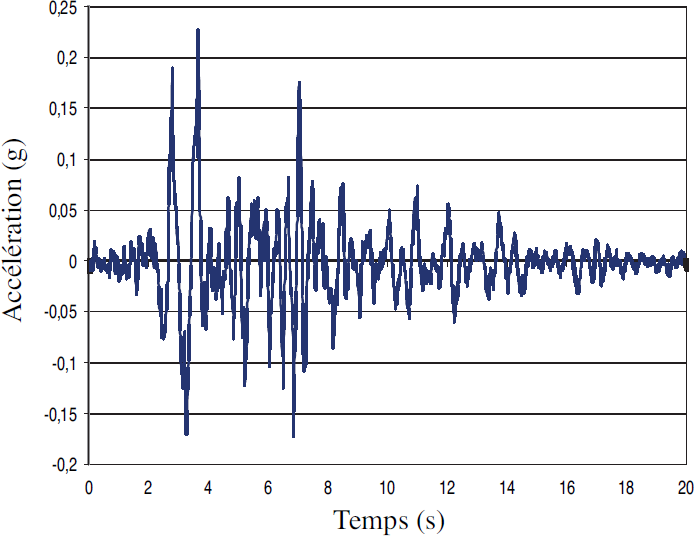
\includegraphics[width=\textwidth]{fig_02}
\end{center}

\textbf{Remarque :} en ajoutant l'hypothèse en début de partie II.B.1, l'action de 7 sur 3 est modélisée par un couple. Dans ce cas, le résultat attendu est peut-être 1 inconnue entre 7 et 3.
%
%\begin{center}
%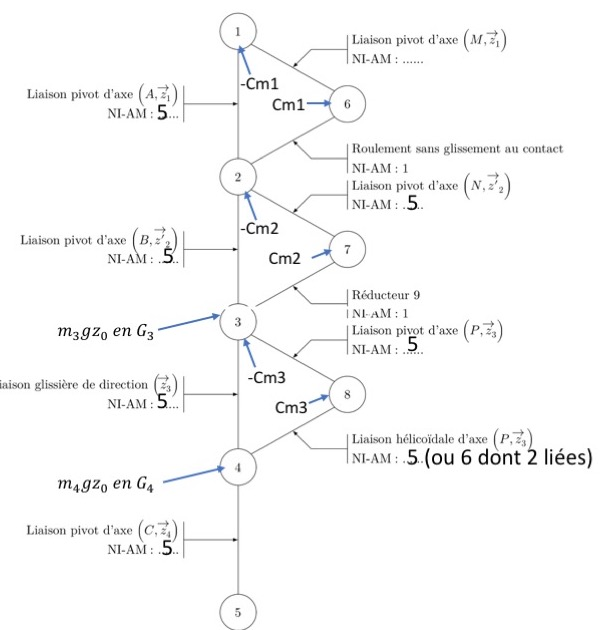
\includegraphics[width=0.8\textwidth]{graphe_structure_complet.jpg}
%\end{center}
\question{}%17
On cherche à déterminer le couple $C_{m2}$ à fournir sur l'arbre 7. L'arbre 7 est en rotation autour de l'axe $\axe{N}{z_2'}$. Il entraîne l'ensemble $\left\{3+8+4+5\right\}$ en rotation autour de l'axe $\axe{B}{z_2'}$.

\begin{center}
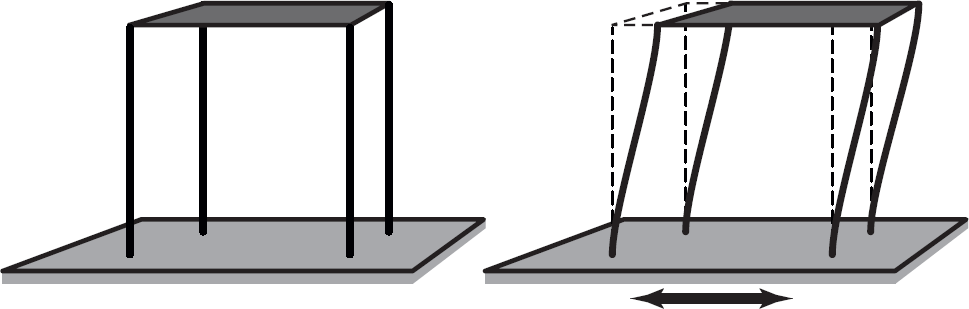
\includegraphics[width=\textwidth]{fig_05}
\end{center}

On propose donc les isolements et des théorèmes associés suivants : 
\begin{itemize}
\item isolement de $\left\{3+8+4+5\right\}$ : théorème du moment dynamique en projection sur $\left(B,\overrightarrow{z}_2'\right)$ qui permet de relier l'action de 7 sur 3 aux paramètres de mouvement de l'ensemble $\left\{3+8+4+5\right\}$ qui représente dans le cas particulier du mouvement souhaité la même classe d'équivalence;
\item isolement de $7$ : théorème du moment dynamique selon $\left(N,\overrightarrow{z}_2'\right)$ qui revient à un théorème du moment statique car l'inertie de 7 est négligeable. Cela permet de relier $C_{m2}$ à l'action de 3 sur 7.
\end{itemize}
Cet ordonnancement des isolements permet de ne pas faire apparaître les inconnues dans les liaisons pivot entre 2 et 7 ainsi qu'entre 7 et 3. 


\question{}%18 --
On cherche $\vectv{G_4}{4}{1}$. On a $\vect{OG_4}=\vect{OA}+\vect{AB}+\vect{BC}+\vect{CG_4}$ $=l_0\vect{y_0}+l_1\vect{y_1}+l_2\vect{y_2}+l_2'\vect{y_2'}+l_3\vect{y_3}+\lambda(t)\vect{z_3}+b_4\vect{z_4}$.
On a $\alpha_1=\dfrac{\pi}{4}$ et $\alpha_2=-\dfrac{\pi}{4}$.

On a donc $\vectv{G_4}{4}{1}= \left[\dfrac{\dd \vect{OG_4}}{\dd t}\right]_{\rep{0}} $ 

$= 
\left[\dfrac{\dd l_0\vect{y_0}}{\dd t}\right]_{\rep{0}}+
\left[\dfrac{\dd l_1\vect{y_1}}{\dd t}\right]_{\rep{0}}+
\left[\dfrac{\dd l_2\vect{y_2}}{\dd t}\right]_{\rep{0}}+
\left[\dfrac{\dd l_2'\vect{y_2'}}{\dd t}\right]_{\rep{0}}+
\left[\dfrac{\dd l_3\vect{y_3}}{\dd t}\right]_{\rep{0}}+
\left[\dfrac{\dd \lambda(t)\vect{z_3}}{\dd t}\right]_{\rep{0}}+
\left[\dfrac{\dd b_4\vect{z_4}}{\dd t}\right]_{\rep{0}}$

$= 
\vect{0}+
\vect{0}+
l_2\left[\dfrac{\dd \vect{y_2}}{\dd t}\right]_{\rep{0}}+
l_2'\left[\dfrac{\dd \vect{y_2'}}{\dd t}\right]_{\rep{0}}+
l_3\left[\dfrac{\dd \vect{y_3}}{\dd t}\right]_{\rep{0}}+
\lambda(t)\left[\dfrac{\dd \vect{z_3}}{\dd t}\right]_{\rep{0}}+
\dot{\lambda}(t)\left[\dfrac{\dd \vect{z_3}}{\dd t}\right]_{\rep{0}}+
b_4\left[\dfrac{\dd \vect{z_4}}{\dd t}\right]_{\rep{0}}$

$= 
l_2\left[ \vecto{2}{0} \wedge \vect{y_2} \right]+
l_2'\left[ \vecto{2'}{0} \wedge \vect{y_2'} \right]+
l_3\left[ \vecto{3}{0} \wedge \vect{y_3} \right]+
\lambda(t)\left[ \vecto{3}{0} \wedge \vect{z_3} \right]+
\dot{\lambda}(t)\vect{z_3}+
b_4\left[ \vecto{4}{0} \wedge \vect{z_4} \right]$. 

$= 
l_2\left[ \dot{\theta}_{21}\vect{z_2} \wedge \vect{y_2} \right]+
l_2'\left[ \dot{\theta}_{21}\vect{z_2} \wedge \vect{y_2'} \right]+
l_3\left[ \left(\dot{\theta}_{21}\vect{z_2}+\dot{\theta}_{32}\vect{z_3} \right) \wedge \vect{y_3} \right]+
\lambda(t)\left[ \left(\dot{\theta}_{21}\vect{z_2}+\dot{\theta}_{32}\vect{z_3} \right) \wedge \vect{z_3} \right]+
\dot{\lambda}(t)\vect{z_3}+
b_4\left[ \left(\dot{\theta}_{21}\vect{z_2}+\dot{\theta}_{32}\vect{z_3} \right) \wedge \vect{z_3} \right]$. 

Or $\dot{\theta}_{21}=0$. On a donc :
$\vectv{G_4}{4}{1}= 
l_3\left(\dot{\theta}_{32}\vect{z_3} \wedge \vect{y_3} \right)+
\dot{\lambda}(t)\vect{z_3} =
-\dot{\theta}_{32}l_3\vect{x_3}  + \dot{\lambda}(t)\vect{z_3}$.

%
%$= 
%-l_2 \dot{\theta}_{21}\vect{x_2} 
%-l_2'\dot{\theta}_{21}\cos \alpha_2\vect{x_2}+
%l_3\left[ \dot{\theta}_{21}\vect{z_2}\wedge \vect{y_3}-\dot{\theta}_{32}\vect{x_3}  \right]+
%\lambda(t) \dot{\theta}_{21}\sin \alpha_2\vect{x_2} +
%\dot{\lambda}(t)\vect{z_3}+ b_4\dot{\theta}_{21}\sin \alpha_2\vect{x_2}$. 
%
%
%Par ailleurs, 
%$\vect{z_2}\wedge \vect{y_3}=\vect{z_2}\wedge \left( \cos \theta_{32} \vect{y_2'} -\sin \theta_{32} \vect{x_2'}  \right)$
%$= \cos \theta_{32} \vect{z_2}\wedge  \vect{y_2'} -\sin \theta_{32} \vect{z_2}\wedge\vect{x_2'}  $
%$= -\cos \theta_{32} \cos \alpha_2 \vect{x_2'} -\sin \theta_{32} \vect{y_2}  $.
%
%Au final, on a 
%
%$\vectv{G_4}{4}{1}=
%-l_2 \dot{\theta}_{21}\vect{x_2} 
%-l_2'\dot{\theta}_{21}\cos \alpha_2\vect{x_2}+
%l_3\left[ \dot{\theta}_{21}\left(-\cos \theta_{32} \cos \alpha_2 \vect{x_2'} -\sin \theta_{32} \vect{y_2}  \right)-\dot{\theta}_{32}\vect{x_3}  \right]+
%\lambda(t) \dot{\theta}_{21}\sin \alpha_2\vect{x_2} +
%\dot{\lambda}(t)\vect{z_3}+ b_4\dot{\theta}_{21}\sin \alpha_2\vect{x_2}$.
%

%En tenant compte de l'hypothèse $\dot{\theta}_{21}=0$, on a : $\vectv{G_4}{4}{1}=
%-\dot{\theta}_{32}l_3\vect{x_3}  + \dot{\lambda}(t)\vect{z_3}$.


\question{}%19 --
En utilisant l'évolution de $\dot{\theta}_{32}$, on peut déterminer le déplacement angulaire effectué en traçant l'aire sous la courbe :
$\theta_{32}=\dfrac{1}{2}\left( 1+0,5\right)\times 0,075 =\SI{0,056}{rad}\simeq 3^{\text{o}}$.

Cet angle étant faible, on peut donc considérer que $\forall t \cos \left(\theta_{32}(t)\right)\simeq 1$ et $\sin\left(\theta_{32}(t)\right)\simeq 0$.

\question{}%20 -- 

On donne $J_4$ le moment d'inertie du bras 4 autour de l'axe $\axe{G_4}{z_4}$.

\textbf{Méthode}
\begin{enumerate}
\item Expression de $\vectmd{B}{4}{1}\cdot\vect{z_4} = \left( \vectmd{G_4}{4}{1} + \vect{BG_4}\wedge m_4 \vectg{G_4}{4}{1}\right)\cdot\vect{z_4}$.
\item Calcul de $\vectmd{G_4}{4}{1}$.
\end{enumerate}

$\vectmd{G_4}{4}{1} \cdot\vect{z_4} = \left[ \dfrac{\dd \vectmc{G_4}{4}{1}}{\dd t} \right]_{\rep{0}}\cdot\vect{z_4}
=\left[ \dfrac{\dd \vectmc{G_4}{4}{1}\cdot \vect{z_4}}{\dd t} \right]-\vectmc{G_4}{4}{1}\cdot\left[ \dfrac{\dd \vect{z_4}}{\dd t} \right]_{\rep{0}}$



On a $\vectmc{G_4}{4}{1} =\inertie{G_4}{4} \vecto{4}{1}$ avec $\vecto{4}{1}=\underbrace{\vecto{4}{3}}_{\vect{0}}+\vecto{3}{2}+\vecto{2}{1} =\dot{\theta}_{32} \vect{z_3}+\underbrace{\dot{\theta}_{21}}_{0} \vect{z_2}=\dot{\theta}_{32} \vect{z_4}$.

Donc,
$\vectmc{G_4}{4}{1}\cdot\vect{z_4}=J_4\dot{\theta}_{32} $.

De plus, $ \left[ \dfrac{ \dd \vect{z_4}}{\dd t} \right]_{\rep{0}} = \vect{0} $. 
En conséquences, $\vectmd{G_4}{4}{1} \cdot\vect{z_4}  = J_4\ddot{\theta}_{32}$.

Par ailleurs, $\vectg{G_4}{4}{1}= \left[\dfrac{\dd \vectv{G_4}{4}{1}}{\dd t} \right]_{\rep{0}}=\left[\dfrac{\dd \left( -\dot{\theta}_{32}l_3\vect{x_3}  + \dot{\lambda}(t)\vect{z_3} \right)}{\dd t} \right]_{\rep{0}}$
$= -\ddot{\theta}_{32}l_3\vect{x_3} -\dot{\theta}_{32}l_3    \left(\dot{\theta}_{32} \vect{z_3}\wedge \vect{x_3} \right)  + \ddot{\lambda}(t)\vect{z_3}  $

$= -\ddot{\theta}_{32}l_3\vect{x_3} -l_3   \dot{\theta}_{32}^2  \vect{y_3} + \ddot{\lambda}(t)\vect{z_3}  $.

$\left(\vect{BG_4}\wedge m_4 \vectg{G_4}{4}{1}\right)\cdot\vect{z_4} = 
m_4\left( \left(l_3 \vect{y_3} + \lambda(t) \vect{z_3}+ b_4 \vect{z_4}\right) \wedge  \left(-\ddot{\theta}_{32}l_3\vect{x_3} -l_3   \dot{\theta}_{32}^2  \vect{y_3} + \ddot{\lambda}(t)\vect{z_3} \right) \right)\cdot \vect{z_{4,3}}$

Par simplification avec les propriétés du produit mixte et du produit vectoriel,

$
\left(\vect{BG_4}\wedge m_4 \vectg{G_4}{4}{1}\right)\cdot\vect{z_4} =
m_4\left( \left(l_3 \vect{y_3} \right) \wedge  \left(-\ddot{\theta}_{32}l_3\vect{x_3} \right) \right)\cdot \vect{z_{4,3}}
=m_4\cdot l_3^2\ddot{\theta}_{32}
$


  Au final,  $\vectmd{B}{4}{1}\cdot\vect{z_4} = J_4 \ddot{\theta}_{32}+\ddot{\theta}_{32}l_3^2 m_4 $.
  



%
%$= m_4\left( \left(l_3 \vect{y_3} + \lambda(t) \vect{z_3}+ b_4 \vect{z_4}\right) \wedge  \left(-\ddot{\theta}_{32}l_3\vect{x_3}\right)  + \left(l_3 \vect{y_3} + \lambda(t) \vect{z_3}+ b_4 \vect{z_4}\right) \wedge  \left(-l_3   \dot{\theta}_{32}^2  \vect{y_3}\right) + \left(l_3 \vect{y_3} + \lambda(t) \vect{z_3}+ b_4 \vect{z_4}\right) \wedge  \left(\ddot{\lambda}(t)\vect{z_3}\right) \right) \cdot \vect{z_4}$
%
%$= m_4\left(\left( \left(l_3 \vect{y_3} + \lambda(t) \vect{z_3}+ b_4 \vect{z_4}\right) \wedge  \left(-\ddot{\theta}_{32}l_3\vect{x_3}\right) \right) \cdot \vect{z_4} 
% + \left(\left(l_3 \vect{y_3} + \lambda(t) \vect{z_3}+ b_4 \vect{z_4}\right) \wedge  \left(-l_3   \dot{\theta}_{32}^2  \vect{y_3}\right)\right) \cdot \vect{z_4}
%  +\left( \left(l_3 \vect{y_3} + \lambda(t) \vect{z_3}+ b_4 \vect{z_4}\right) \wedge  \left(\ddot{\lambda}(t)\vect{z_3}\right) \right) \cdot \vect{z_4}\right)$
%  
%$= m_4\left(\left( \vect{z_4} \wedge  \left(l_3 \vect{y_3} + \lambda(t) \vect{z_3}+ b_4 \vect{z_4}\right)  \right) \cdot  \left(-\ddot{\theta}_{32}l_3\vect{x_3}\right)
% + \left(\vect{z_4} \wedge \left(l_3 \vect{y_3} + \lambda(t) \vect{z_3}+ b_4 \vect{z_4}\right)  \right) \cdot \left(-l_3   \dot{\theta}_{32}^2  \vect{y_3}\right)
%  +\left( \vect{z_4} \wedge \left(l_3 \vect{y_3} + \lambda(t) \vect{z_3}+ b_4 \vect{z_4}\right) \right) \cdot   \left(\ddot{\lambda}(t)\vect{z_3}\right) \right)$
%  
%  $= m_4\left(\left( \vect{z_4} \wedge  l_3 \vect{y_3}  \right) \cdot  \left(-\ddot{\theta}_{32}l_3\vect{x_3}\right)   \right)$
%
%  $= \ddot{\theta}_{32}l_3^2 m_4 $.
  



\question{}%21 --


Par analogie avec la question précédente, on a $\vectmd{B}{3}{1}\cdot\vect{z_4}= J_3\ddot{\theta}_{32}+\ddot{\theta}_{32}a_3^2 m_3$.

En conséquence,  $\vectmd{B}{3+4+5+8}{1}\cdot\vect{z_4} = \left(J_3+J_4+a_3^2 m_3  +l_3^2 m_4\right) \ddot{\theta}_{32}$.

\begin{rem}
On fait l'hypothèse ici que l'action de 3 sur 7 ou du réducteur sur 7 est bien modélisée par une action mécanique de type couple comme le suggère l'énoncé.
\end{rem}



\textbf{On isole l'ensemble $\{3,4,5,8\}$.}

\begin{rem}
Le schéma peut être trompeur car représenté dans une configuration particulière mais la pesanteur crée un moment en $B$ suivant $\vect{z_0}$.
\end{rem}

\begin{itemize}
\item On réalise le bilan des actions mécaniques extérieures. 
\begin{itemize}
\item Action de la pesanteur sur 3 : 
$\vectm{B}{\text{pes}}{3}\cdot \vect{z_4} $ $ =\left(\vect{BG_3}\wedge \left(-m_3g \vect{z_0}\right) \right)\vect{z_4}$ 
$ =\left(\left( a_3\vect{y_3} + b_3\vect{z_3}  \right)\wedge \left(-m_3g \vect{z_0}\right)\right)\vect{z_4}$
$ =\left( a_3\vect{y_4} \wedge \left(-m_3g \vect{z_0}\right)\right)\vect{z_4}$
$ =\left( \vect{z_4} \wedge a_3\vect{y_4}\right)\cdot  \left(-m_3g \vect{z_0}\right)$
$ = a_3 m_3g \left( \vect{x_3}\cdot \vect{z_0} \right)$
$ = a_3 m_3g \left(  \cos\theta_{32} \vect{x_2'} +\sin\theta_{32} \vect{y_2'} \right)\cdot \vect{z_0} $

On utilise les hypothèses de linéarisation vues précédemment et on a 
$\vectm{B}{\text{pes}}{3}\cdot \vect{z_4}= a_3 m_3g \vect{x_2'} \cdot \vect{z_0} $ 
$= a_3 m_3g \vect{x_2} \cdot \vect{z_0} $
$= a_3 m_3g \left( \cos \theta_{21} \vect{x_1} +\sin \theta_{21} \vect{y_1} \right)\cdot \vect{z_0} $
$= a_3 m_3g \left( \cos \theta_{21} \vect{x_0} +\sin \theta_{21}  \left( \cos \alpha_1 \vect{y_0} + \sin \alpha_1 \vect{z_0} \right) \right)\cdot \vect{z_0} $
$= a_3 m_3g \sin \theta_{21}   \sin \alpha_1    $. En faisant l'application numérique, on a donc 
$\vectm{B}{\text{pes}}{3}\cdot \vect{z_4}= a_3 m_3g  \dfrac{\sqrt{2}}{2} \dfrac{\sqrt{3}}{2}$

\item Action de la pesanteur sur 4 : 
$\vectm{B}{\text{pes}}{4}\cdot \vect{z_4} $ $ =\left(\vect{BG_4}\wedge \left(-m_4g \vect{z_0}\right) \right)\vect{z_4}$ 

$ =\left(\left(l_3\vect{y_3} + \lambda(t) \vect{z_{3,4}} + b_4\vect{z_{3,4}} \right)\wedge \left(-m_4g \vect{z_0}\right) \right)\vect{z_{3,4}}
=\overrightarrow{z}_{3,4}\wedge l_3\overrightarrow{y}_3\cdot \left(-m_4\cdot g\cdot \overrightarrow{z}_0\right)=m_4l_3g\overrightarrow{x}_3\cdot \overrightarrow{z}_0
$

Or,

$\overrightarrow{x}_3=\cos\theta_{32}\overrightarrow{x}_{2,2'}+\sin\theta_{32}\overrightarrow{y}_{2'}$

avec $\cos\theta_{32}\approx 1$ et $\sin\theta_{32}\approx 0$

 Donc, 
 
 $\overrightarrow{x}_3\cdot \overrightarrow{z}_0=\left(\cos\theta_{21}\overrightarrow{x}_{1,0}+\sin\theta_{21}\overrightarrow{y}_1\right)\cdot \overrightarrow{z}_0=\sin\theta_{21}\sin\alpha_1=\dfrac{\sqrt{6}}{4}$
 On obtient alors,
 
 $\vectm{B}{\text{pes}}{4}\cdot \vect{z_4} = =l_3 m_4g\sin\theta_{21}\sin\alpha_1 =l_3 m_4g  \dfrac{\sqrt{6}}{4}$.




\item $\vectm{B}{2}{3}\cdot \vect{z_0}=0$.
\item $\vectm{B}{7}{3}\cdot \vect{z_4}=C_{73}$ (Indication du sujet).
\end{itemize}
\item En appliquant le théorème du moment dynamique en $B$ en projection sur $\vect{z}$ on a donc 
$  \left( a_3^2 m_3  +l_3^2 m_4+J_3+J_4\right) \ddot{\theta}_{32}=C_{73} + g  \sin \theta_{21}   \sin \alpha_1 \left( a_3 m_3 + l_3 m_4\right) $.
\end{itemize}

\textbf{Il semblerait que ce qui est attendu soit d'utiliser ${C_{73}}=C_{m2}\dfrac{\eta_9}{r_9}$, mais cette relation avait été établie en régime permanent ce qui n'est plus le cas. } 


$\left(J_3+J_4  + a_3^2 m_3  +l_3^2 m_4 \right) \ddot{\theta}_{32} =C_{m2}\dfrac{\eta_9}{r_9}+ g  \sin \theta_{21}   \sin \alpha_1 \left( a_3 m_3 + l_3 m_4\right) $.

Par identification, on a donc :
\begin{itemize}
\item $J_{eq} = J_3+J_4  + a_3^2 m_3  +l_3^2 m_4$;
\item $A  =\dfrac{\eta_9}{r_9}$;
\item $C_r(t)=g  \sin \theta_{21}   \sin \alpha_1 \left( a_3 m_3 + l_3 m_4\right) $.
\end{itemize}

\begin{rem} 
$J_{eq}$ dépendrait aussi de $a_3$ et $m_3$.
\end{rem}


\question{}%22 --



\question{}%23 --



\section{Définition et analyse de la chaîne d’asservissement du robot esclave}
\begin{obj}
Définir le régulateur de la chaîne d’asservissement du robot esclave, analyser ses performances vis-à-vis
des perturbations en se limitant à celles dues aux couples de frottement sec et compléter la chaîne
d’asservissement par la compensation de ces efforts.
\end{obj}

\subsection{Calcul d’un correcteur et analyse partielle des performances de la chaîne d’asservissement}
\begin{obj}
Déterminer un correcteur pour la chaîne d’asservissement de la position angulaire des articulations.
Afin d’aboutir à une démarche générale (indépendante d’une articulation particulière), la loi de commande
sera paramétrée par le moment d’inertie équivalent de l’articulation considérée.
\end{obj}

\question{}%24 --


\question{}%25 --



\subsection{Amélioration des performances par compensation du couple de perturbation}
\begin{obj}
Améliorer les performances de la loi de commande vis-à-vis des couples perturbateurs extérieurs.
\end{obj}

%\begin{center}
%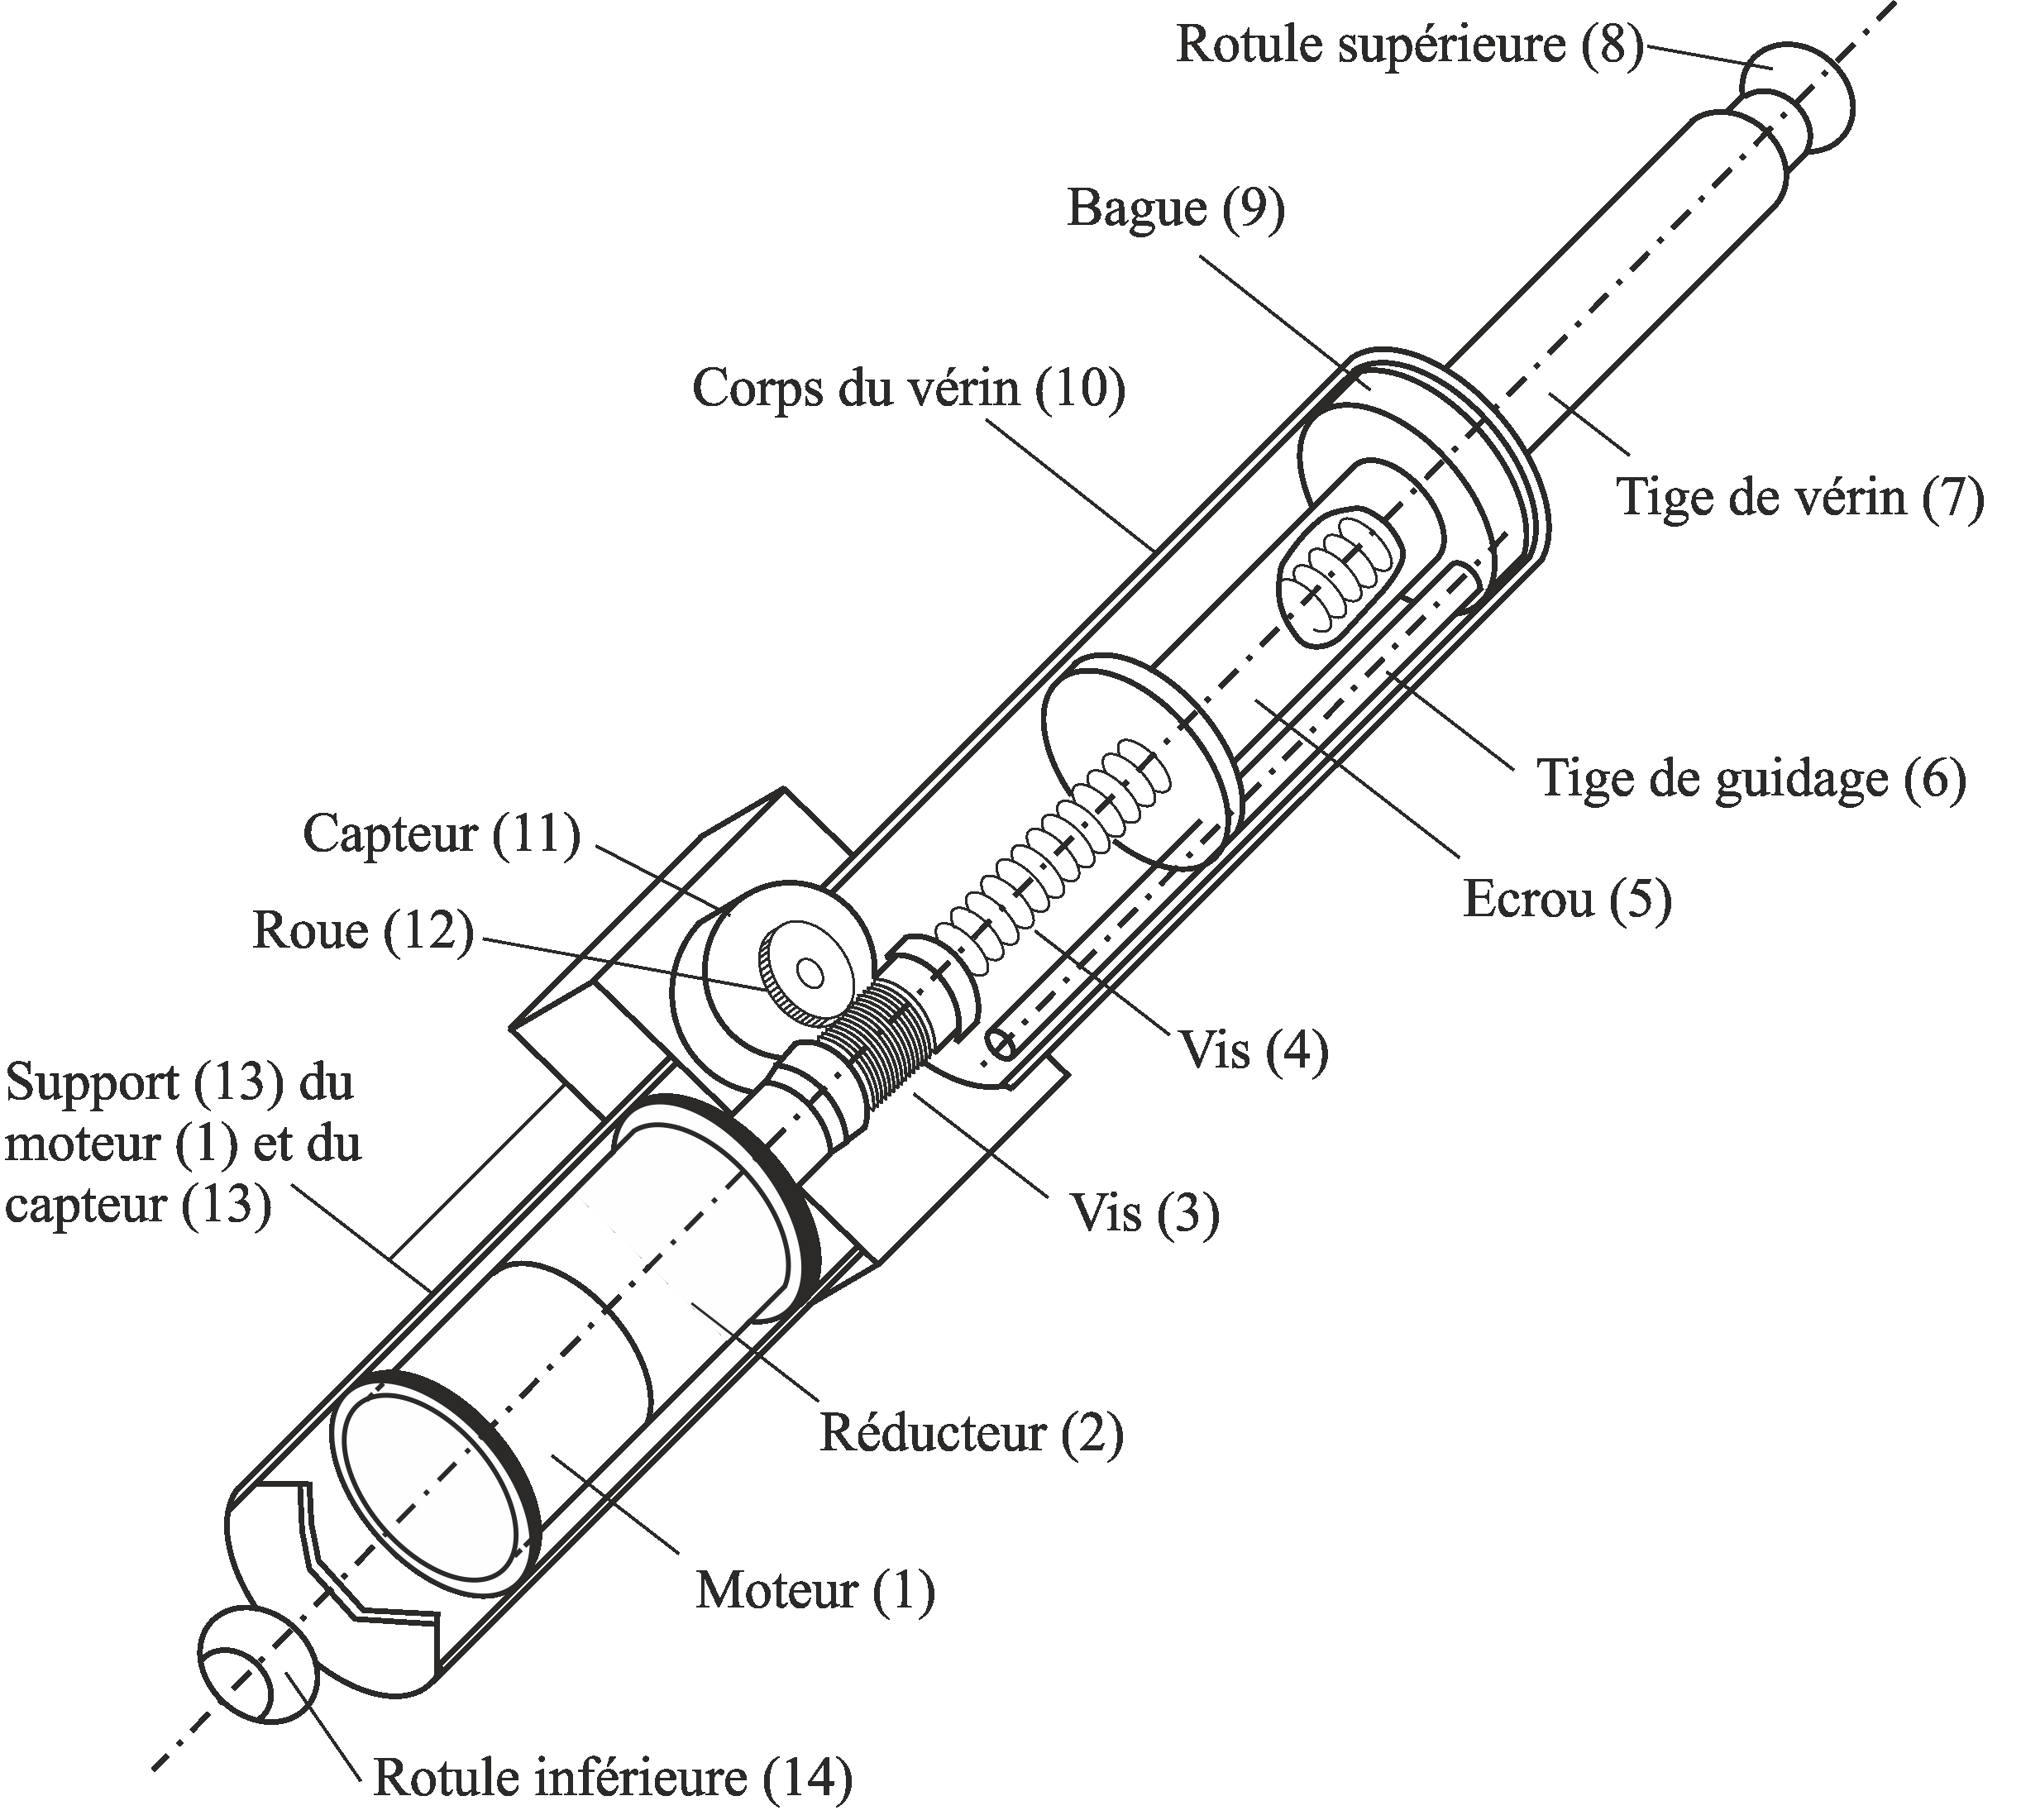
\includegraphics[width=.4\linewidth]{fig_04}
%\end{center}

\question{}%26 --
%On note $A(p)$, $B(p)$ et $C(p)$ les trois fonctions de transfert des trois blocs recherchés. 
%
%
%On a : $Q_j(p)=A(p)\left(C_j(p)+C_{\text{ext}}(p)\right)$, 
%$S(p)=Q_j(p)-B(p)\left( C_j(p)+\hat{C}_{\text{ext}}(p) \right)$
%et  $\hat{C}_{\text{ext}}(p)=C(p)S(p)$.
%
% soit 
%
%$\hat{C}_{\text{ext}}(p)=C(p)\left(Q_j(p)-B(p)\left( C_j(p)+\hat{C}_{\text{ext}}(p) \right)\right)$
%
%$\Leftrightarrow \hat{C}_{\text{ext}}(p) \left(1+ C(p)B(p)\right)=C(p)\left(Q_j(p)-C(p)B(p) \right)$




\question{}%27 --


\question{}%28


\question{}%29





\section{Analyse des performances vis-à-vis des mouvements respiratoires}
\begin{obj}
Quantifier le niveau de performance de la loi de commande déterminée en considérant la consigne
correspondant aux mouvements physiologiques. Une amélioration de la loi de commande est ensuite
envisagée sous la forme d’une anticipation sur la consigne pour améliorer les performances.
\end{obj}


\question{}\textit{}%30


\question{}\textit{}%31


\question{}\textit{}%32


\question{}\textit{}%33



\question{}\textit{}%34



\end{document}




